\section{Estado del arte}

\subsection{Origen de la robótica}
La palabra ``Robótica'' fue acuñada por Isaac Asimov para describir la ciencia que se encarga de estudiar la tecnología de los robots. Procede de las palabras checas robota (trabajo forzado) y robotnik
(sirviente) \cite{ref2}.

El término ``robot'', que procede de la palabra robota, se popularizó gracias a la obra literaria Rossum’s Universal Robot (R.U.R.), escrita por Karel Čapek en 1920 \cite{ref3}.

Según la definición de la Organización Internacional de Estándares (ISO) se considera un robot como un: 

``Mecanismo accionado programable en dos o más ejes con un gradio de autonomía, moviéndose dentro de su entorno, para realizar las tareas previstas'' \cite{ref4}. 


A la hora de hablar del concepto de robótica en general, hay que distinguir entre robótica INDUSTRIAL y robótica de SERVICIO. Esta distinción es fundamental a la hora de su desarrollo, fabricación y comercialización.

Según la norma ISO 8373, la definición de robótica INDUSTRIAL es la siguiente:

``Manipulador multifuncional, controlado automáticamente, reprogramable en tres o más ejes, que puede estar fijo o móvil para uso en aplicaciones de automatización industrial''.

En cuanto a lo que respecta a la robótica de SERVICIO, el Comité ISO TC 184/SC2 lo define como:

``Todo tipo de robot que no es industrial''.

A su vez, la IFR proporciona la siguiente definición:

``Robot que opera de forma parcial o totalmente autónoma al servicio del bienestar de los seres humanos y de equipamientos, excluyendo operaciones manufactureras'' \cite{ref5}.


\subsubsection{Tipos de robots}

Resulta complicado establecer una clasificación exacta de los robots debido a la gran cantidad de ellos que existe, por lo que se pueden clasificar de forma más general según su arquitectura. 

\begin{enumerate}

\item \textbf{Poliarticulados}\\ A este grupo pertenecen los robots cuya característica común es el sedentarismo, aunque pueden ser guiados excepcionalmente para efectuar desplazamientos limitados, y cuya estructura se basa en el movimiento de sus elementos terminales para operar en entornos de trabajo fijos, con uno o más sistemas de coordenadas y con un número determinado de grados de libertad. En este grupo se encuentran principalmente los llamados Robots Industriales,como se muestra en la figura \eqref{figura1}, diseñados para operar en entornos repetitivos y sin interacción humano-robot. También pertenecen los manipuladores y los Robots cartesianos, empleados para abarcar amplias zonas de trabajo, actuar sobre diferentes objetos o reducir el espacio ocupado en el suelo.

\begin{figure}[H]
\centering
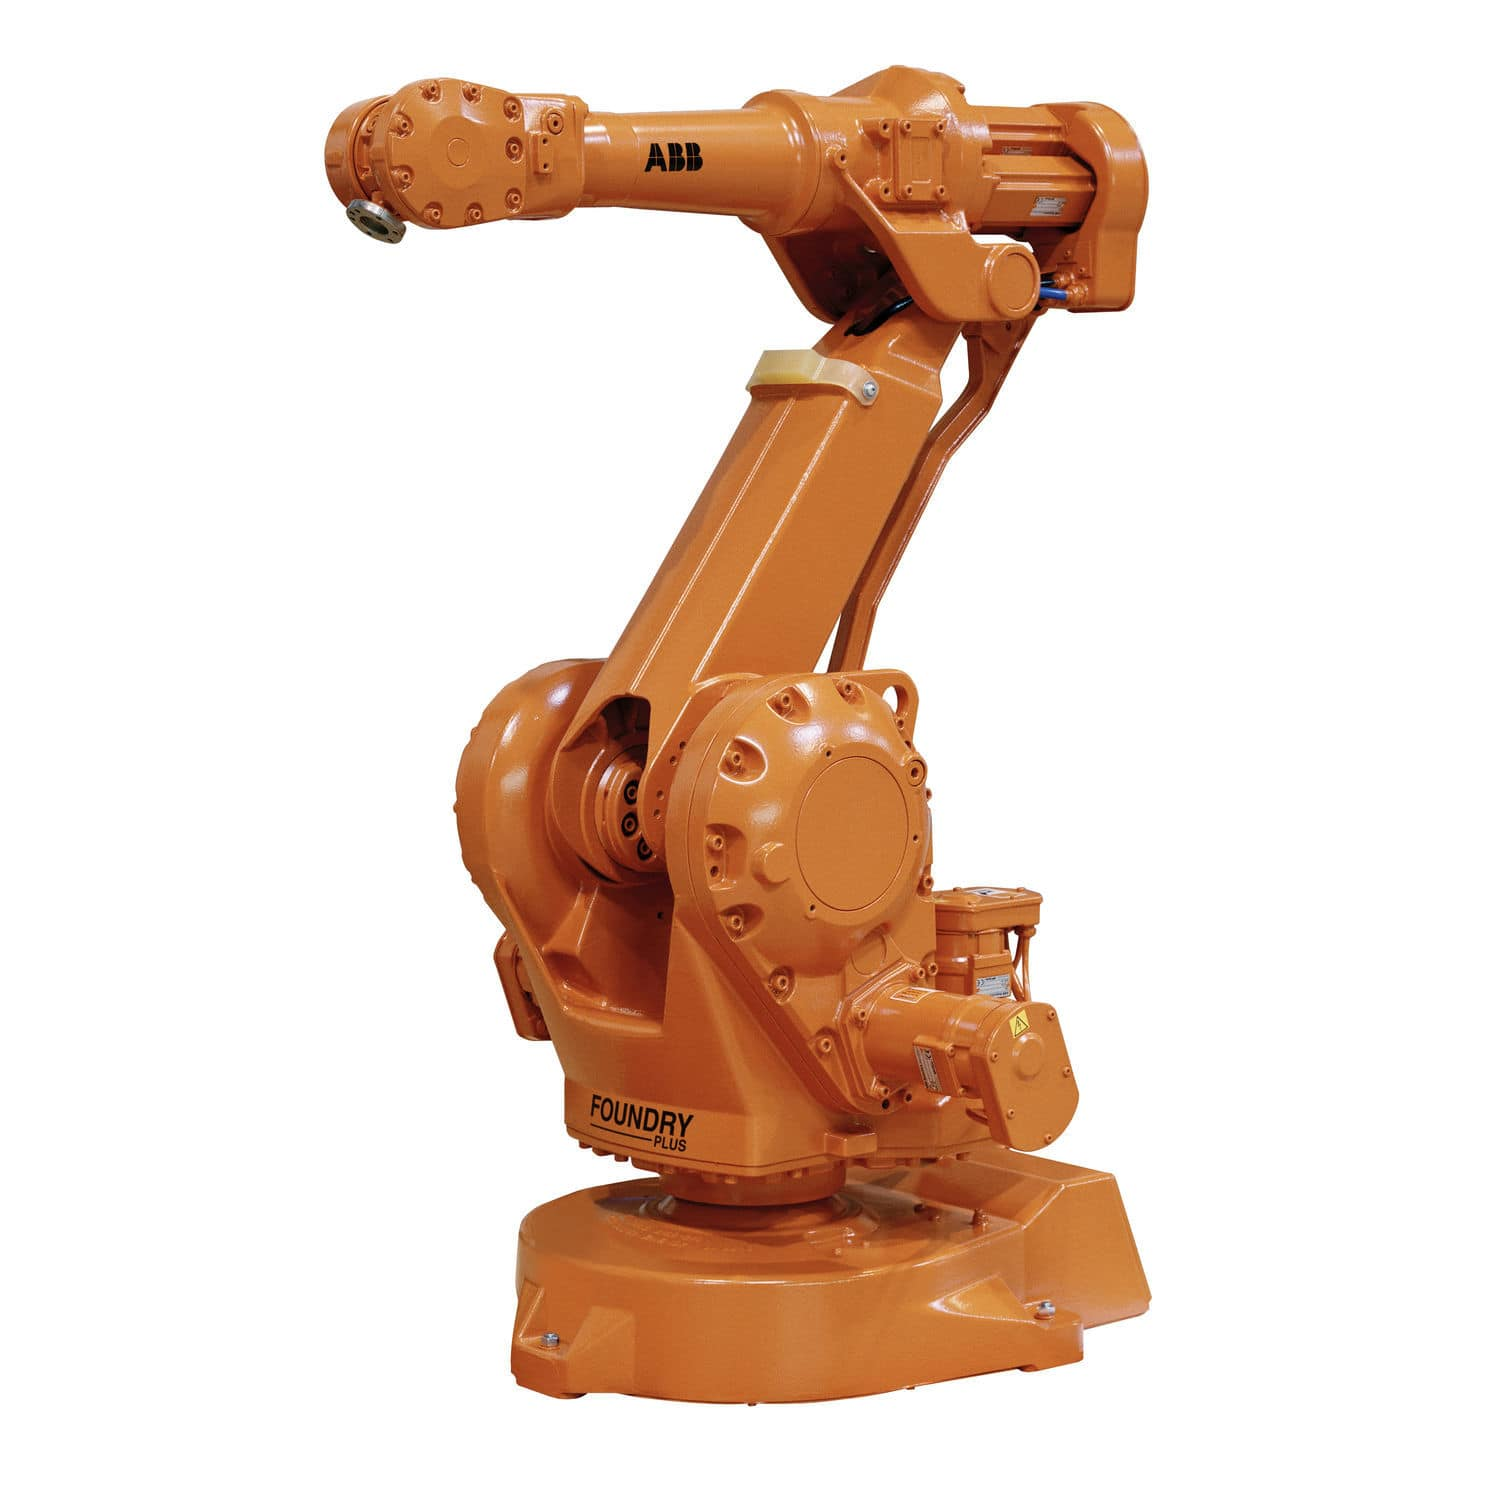
\includegraphics[scale=0.12]{imagenes/apartado_2/21_poliarticulado1_Robot_Industrial_ABB}
\caption{Robot Industrial ABB}
\label{figura21}
\end{figure}

\item \textbf{Móviles}\\ Son robots con capacidad de desplazarse, ya sea mediante ruedas o cualquier plataforma que permita dicha característica, gracias a un sistema motor de tipo rodante. Pueden ser guiados o autónomos (se guían por la información recibida del exterior mediante un sistema de sensores integrado). Estos robots se encargan normalmente de transportar piezas de un punto a otro de la cadena de producción, guiados mediante pistas materializadas a través de la radiación electromagnética de circuitos empotrados en el suelo, o a través de bandas detectadas fotoeléctricamente, otros pueden sortear obstáculos y están dotados de un nivel relativamente elevado de inteligencia.

\begin{figure}[H]
\centering
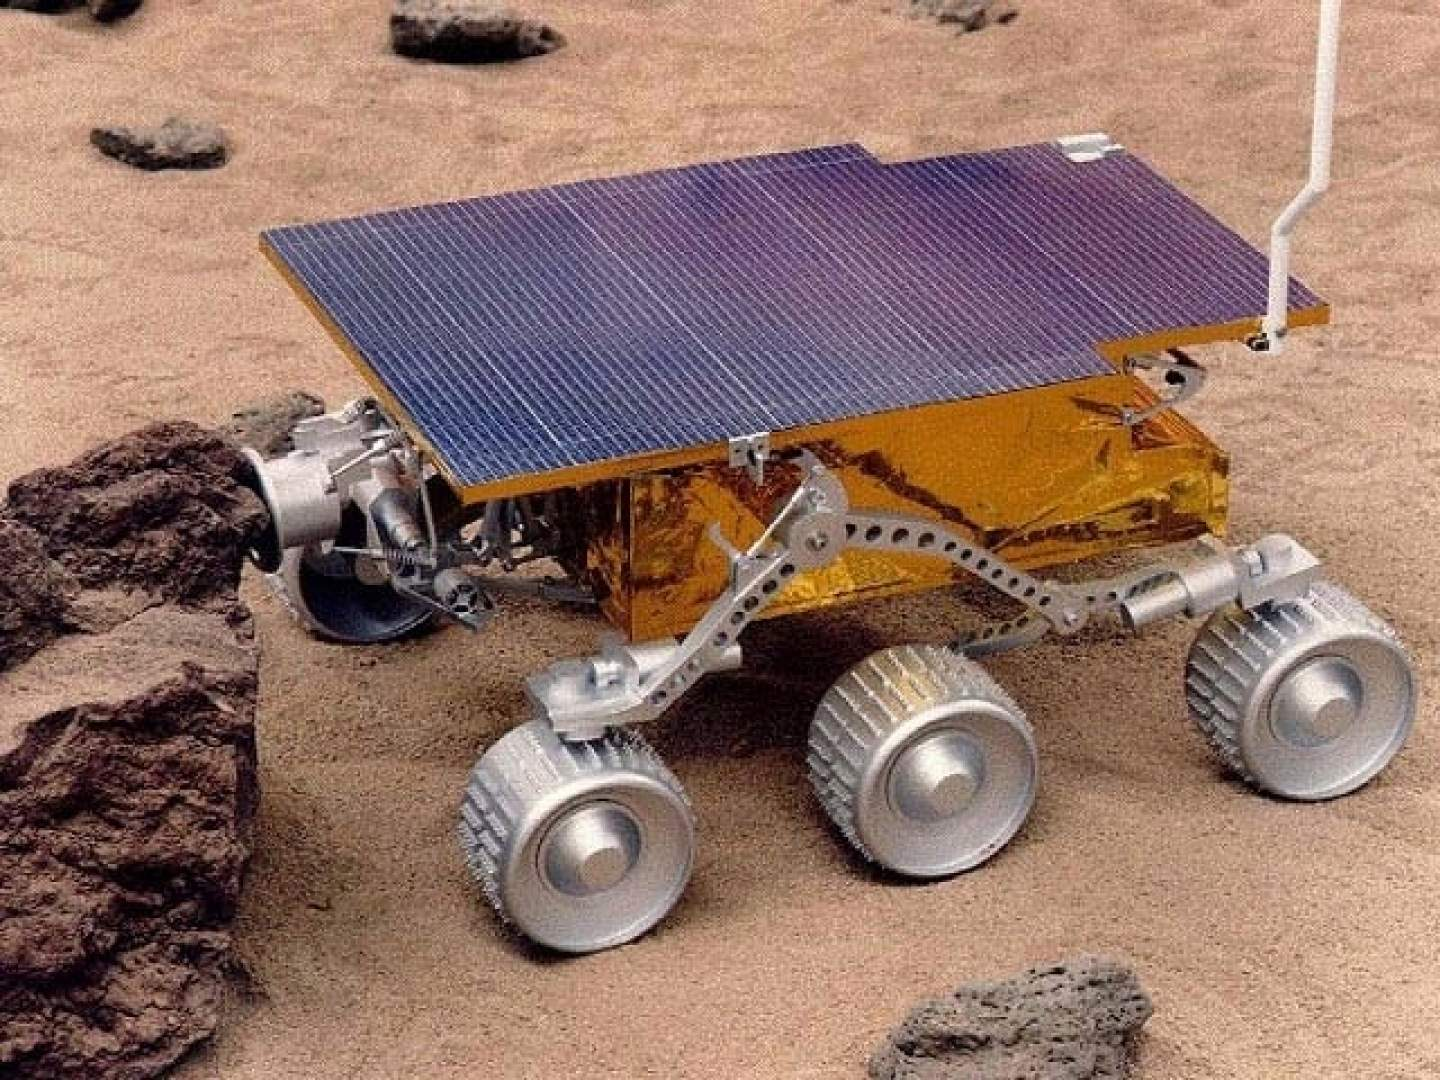
\includegraphics[scale=0.15]{imagenes/apartado_2/22_movil2}
\caption{Mars Pathfinder Rover Sojourner}
\label{figura22}
\end{figure}

\item \textbf{Antropomórficos}\\ Son robots que tratan de imitar parcial o totalmente las acciones y el comportamiento de los seres humanos. Una de las acciones más complejas de éstos es la locomoción bípeda, sobre la que se centra este proyecto y la mayoría de los trabajos en la actualidad, por lo que se concentran en áreas como la investigación y el estudio. El problema que surge es el control dinámico en tiempo real y el mantenimiento simultáneo del equilibrio del robot en dicho proceso.

\begin{figure}[H]
\centering
\subfigure[Robot ASIMO]
{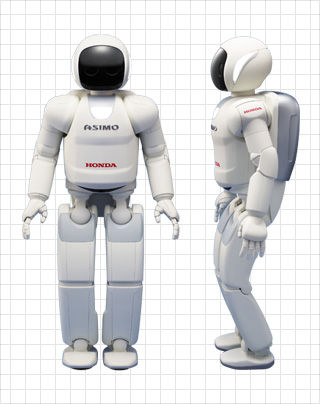
\includegraphics[scale=0.4]{imagenes/apartado_2/23_1_androide1_asimo}}
\quad
\subfigure[Robot TEO]
{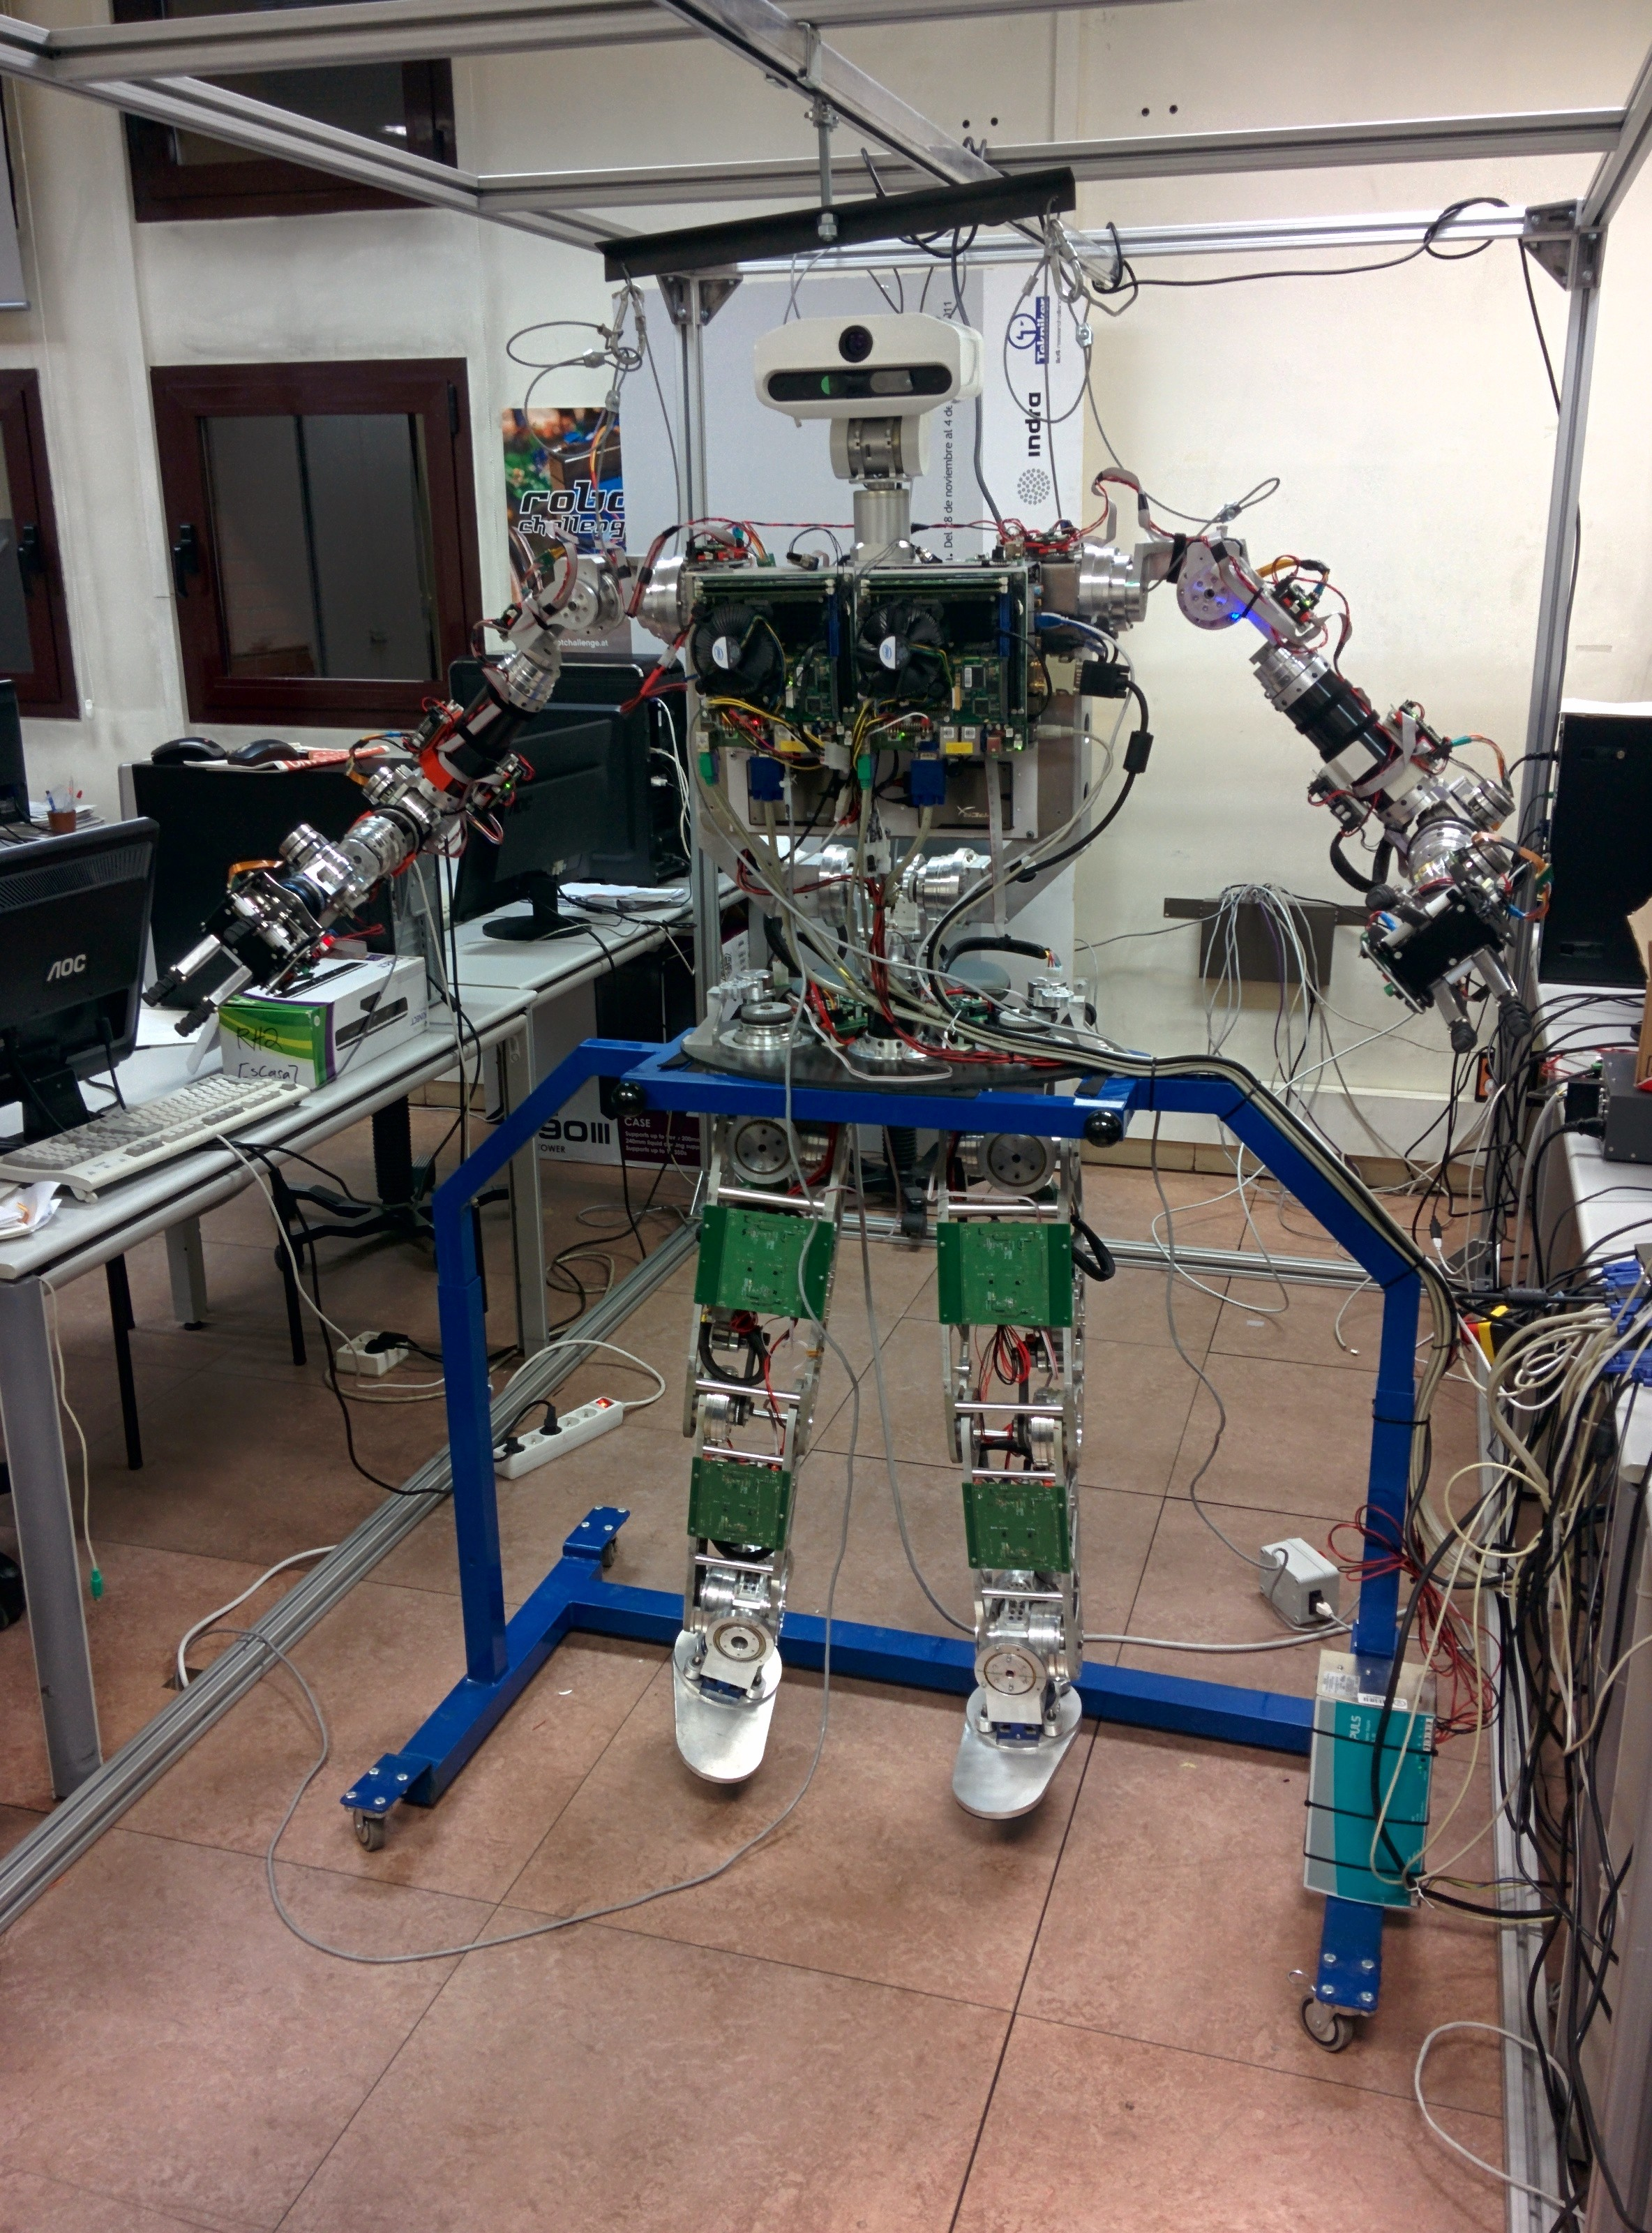
\includegraphics[scale=0.05]{imagenes/apartado_2/23_2_androide2_teo1}}
\caption{Robots antropomórficos}
\label{figura23}
\end{figure}

\item \textbf{Zoomórficos}\\ Son aquellos cuyos sistemas de locomoción imitan a los animales principalmente. Este grupo se podría clasificar en: caminadores y no caminadores.

El grupo de los caminadores es el que más desarrollado está, ya que pueden tener aplicaciones en muchos campos como puede ser el desarrollo de vehículos todoterreno, controlados o autónomos, capaces de avanzar por terrenos con mucho desnivel y accidentados.

Por el contrario, el grupo de los no caminadores es muy escaso y está poco evolucionado. Se han realizado diversos experimentos en Japón con robots de este tipo constituídos por segmentos cilíndricos biselados acoplados axialmente entre sí, capaces de realizar movimientos relativos de rotación.

\begin{figure}[H]
\centering
\subfigure[Robot caminador ANYmal]
{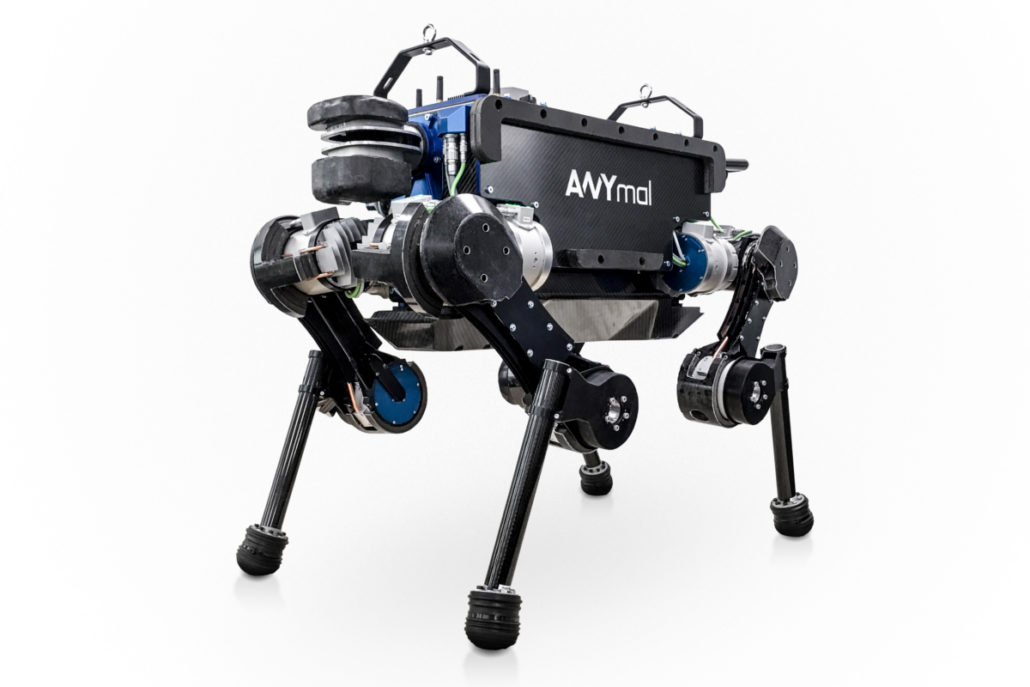
\includegraphics[scale=0.2]{imagenes/apartado_2/24_1_zoomorfico1_ANYmal}}
\quad
\subfigure[Serpiente Robot Modular no caminador]
{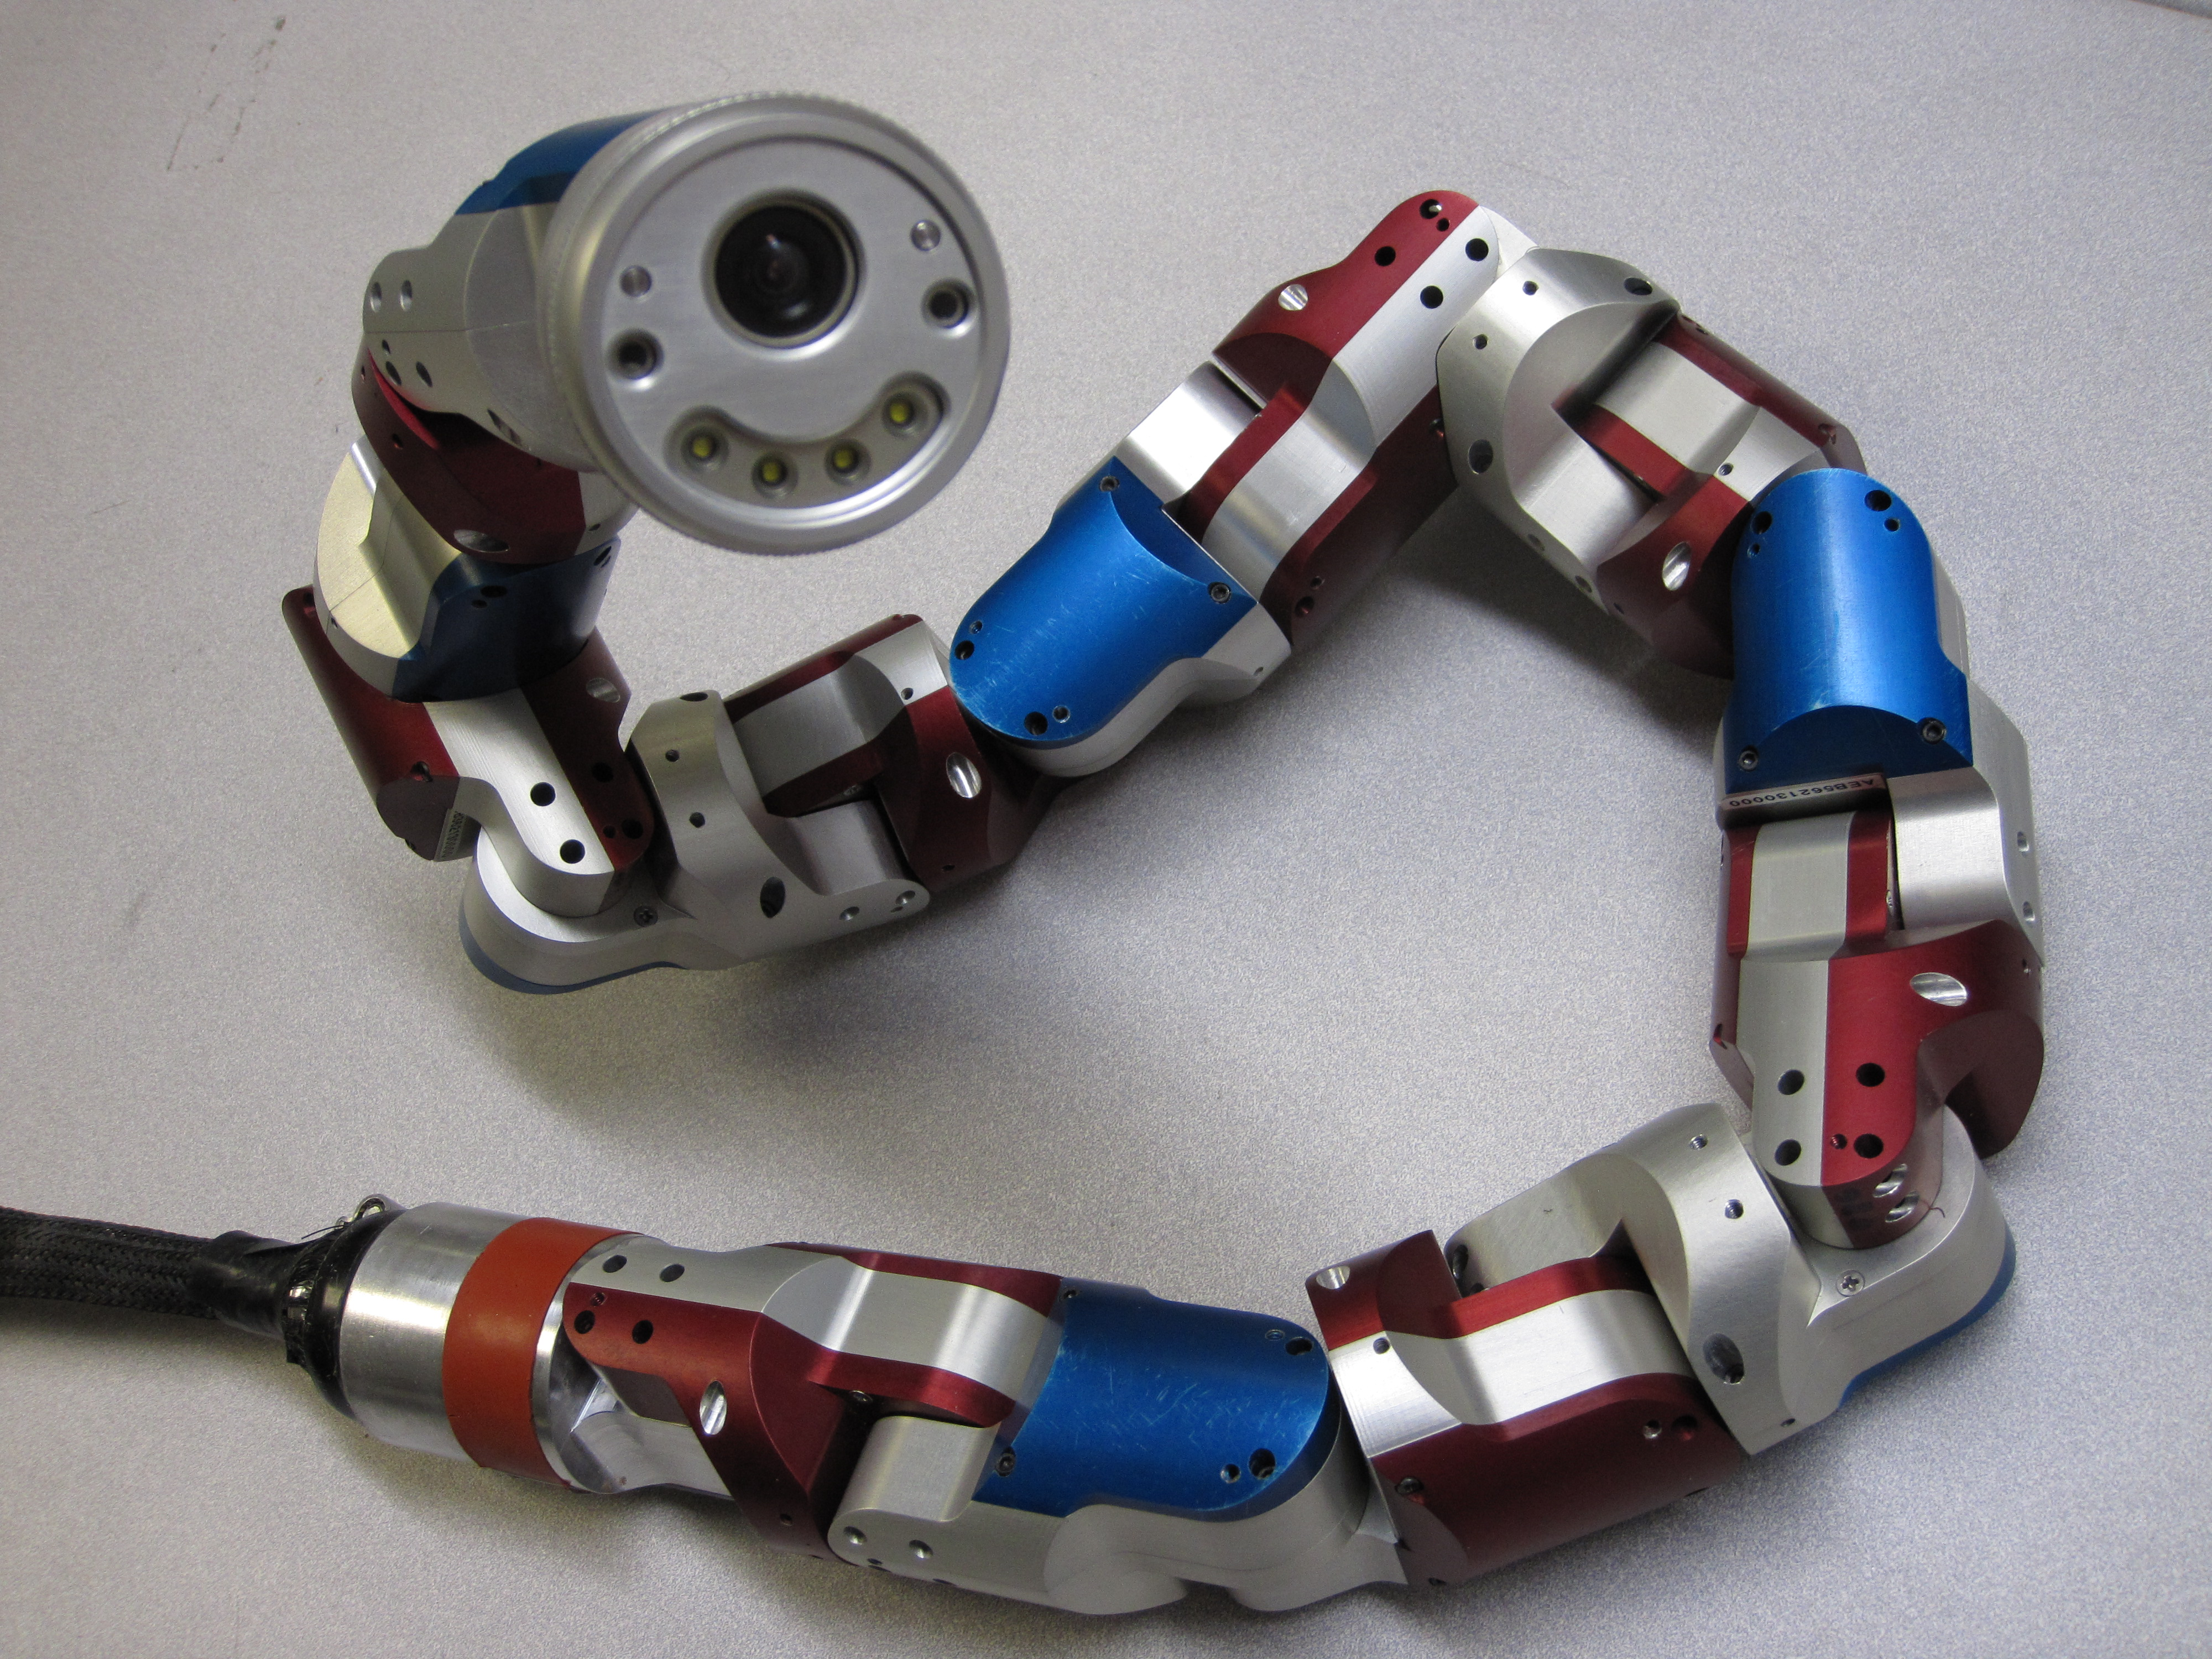
\includegraphics[scale=0.1]{imagenes/apartado_2/24_2_zoomorfico2}}
\caption{Robots zoomórficos}
\label{figura24}
\end{figure} 

\item \textbf{Híbridos}\\ A este grupo pertenecen aquellos Robots que posean en su estructura una combinación de las anteriores ya expuestas, bien sea por conjunción o por yuxtaposición \cite{ref6}. 

Por ejemplo, un dispositivo con ruedas y con brazos, siendo características de los Robots móviles y de los androides al mismo tiempo.

\begin{figure}[H]
\centering
{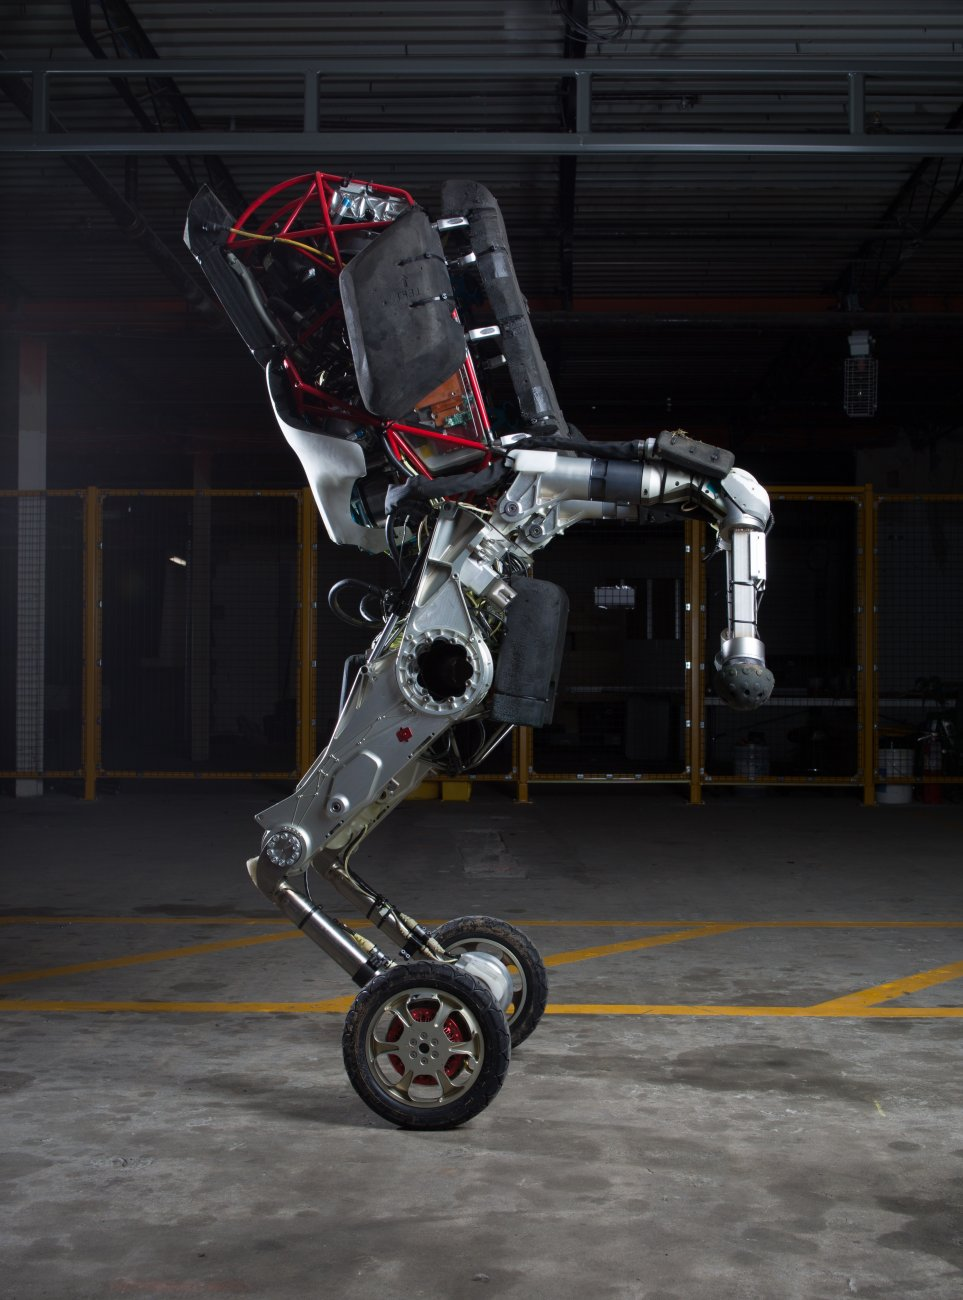
\includegraphics[scale=0.15]{imagenes/apartado_2/25_hibrido_handle_bd}}
\caption{Robot HANDLE}
\label{figura25}
\end{figure}

\end{enumerate}

\newpage

\subsection{Evolución de los Robots Humanoides}

El desarrollo de los robots humanoides ha sido largo y complejo.

Hubo que esperar al año 1495 para tener los primeros registros del que posiblemente sea el primer robot humanoide, diseñado y construído por Leonardo da Vinci. Se trataba de un robot mecánico, un guerrero vestido con una armadura, que podía realizar movimientos similares a los de los seres humanos como sentarse, mover los brazos y girar la cabeza y el cuello \cite{ref7}.

\begin{figure}[H]
\centering
{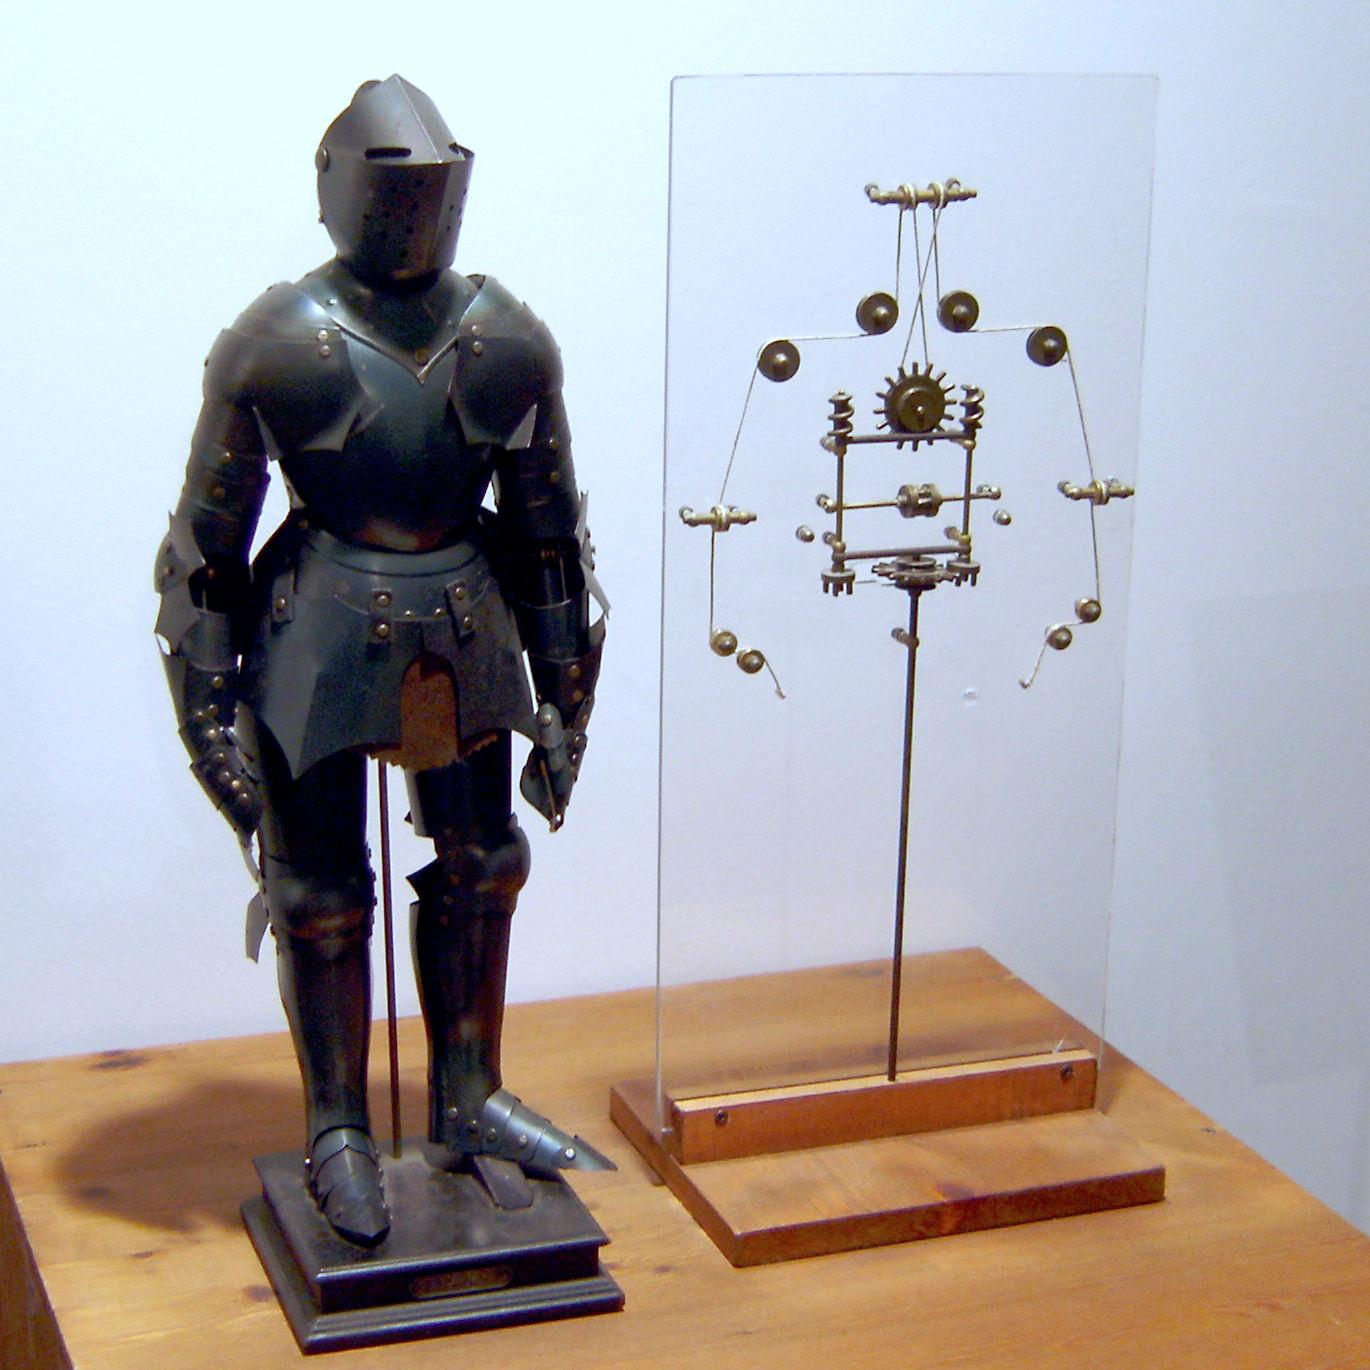
\includegraphics[scale=0.1]{imagenes/apartado_2/26_robot_LeonardoDaVinci}}
\caption{Armadura diseñada por Leonardo Da Vinci}
\label{figura26}
\end{figure}

El siglo XVIII fue una época prolífica para el desarrollo de robots autónomos. En 1773, Pierre y Henry Louis inventaron la primera máquina autónoma capaz de escribir.

Pero cuando empieza realmente el desarrollo de los robots humanoides fue a partir del siglo XIX. Uno de los primeros fue el trompetista mecánico, construido por Fridrich Kaufmann en 1810, que contenía un tambor con muescas que usaba para activar algunas válvulas que ayudaban a pasar el aire a través de doce lenguas, lo que producía un tipo de sonido modulado que a su vez pasaba por una trompeta, para hacerla sonar. En 1865 John Brainerd inventó el hombre de vapor, movido por una máquina de vapor que tiraba de unos carros. En 1855 Frank Reade Junior construyó al llamado Hombre Eléctrico, una versión electrificada del hombre de vapor.

\begin{figure}[H]
\centering
{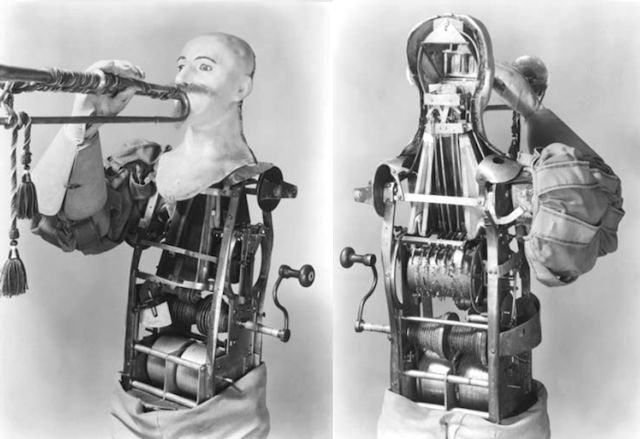
\includegraphics[scale=0.3]{imagenes/apartado_2/27_trompetista_mecanico}}
\caption{Trompetista mecánico}
\label{figura27}
\end{figure}

A partir del siglo XX el número de robots humanoides fue aumentando y evolucionando. Uno de los primeros fue ELEKTRO, desarrollado por la sociedad Westinghouse en 1938, un robot más cerca del concepto de humanoide que podía caminar controlado por comandos de voz, y hablaba gracias a un tocadiscos de 78 rpm. Más tarde se le unió ``Sparko'', un perro robot capaz de sentarse, ladrar y suplicar. 

\begin{figure}[H]
\centering
{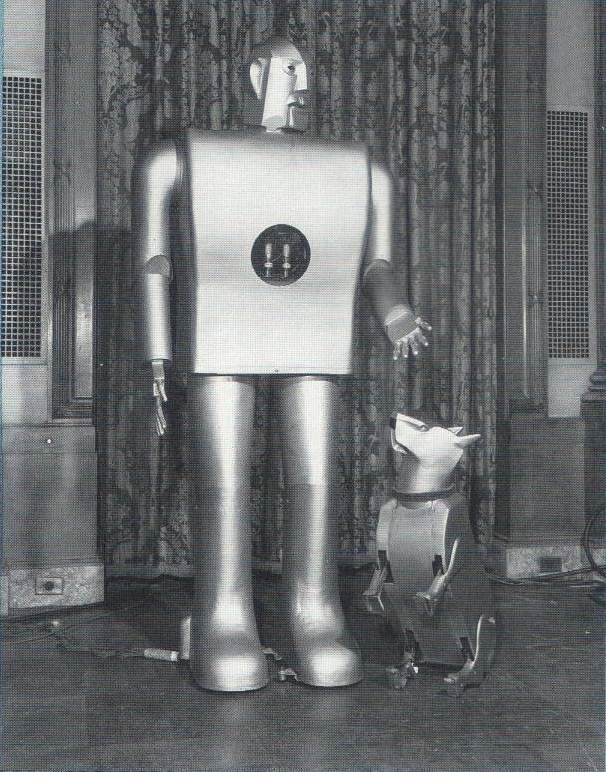
\includegraphics[scale=0.2]{imagenes/apartado_2/28_elektro_robot}}
\caption{Robot Elektro}
\label{figura28}
\end{figure}

Durante las décadas de los 60's a los 90's aparecieron numerosos robots bípedos. El profesor Kato del equipo robótico de la Universidad de Waseda en Japón desarrolló varias familias de robots bípedos.La primera fue llamada Waseda Legged (WL), que se caracterizaba por ser robots compuestos de sólo dos piernas.  En 1969, con la aparición del músculo artificial de goma, desarrollaron la serie WAP (Waseda's Anthropomorphic Pneumatically-activated pedipulators), activados mediante el control de dichos músculos. No fue hasta el modelo WAP-3 que consiguieron que el robot bípedo se desplazara en 3 dimensiones, ya que los dos primeros modelos sólo se movían en un plano.

\begin{figure}[H]
\centering
\subfigure[WL-1]
{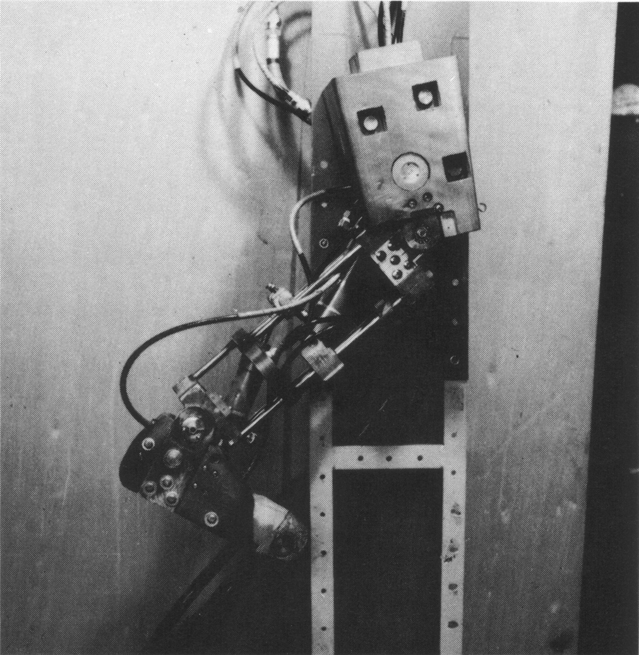
\includegraphics[scale=0.5]{imagenes/apartado_2/29_1_WL_1_1967}}
\quad
\subfigure[WL-3]
{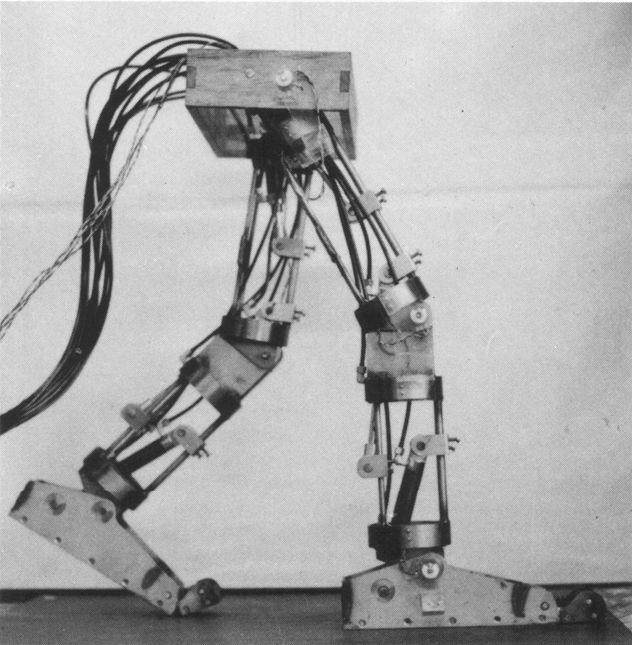
\includegraphics[scale=0.5]{imagenes/apartado_2/29_2_WL_3_1969}}
\caption{Robots Waseda Legged}
\label{figura29}
\end{figure}

\begin{figure}[H]
\centering
\subfigure[WAP-1]
{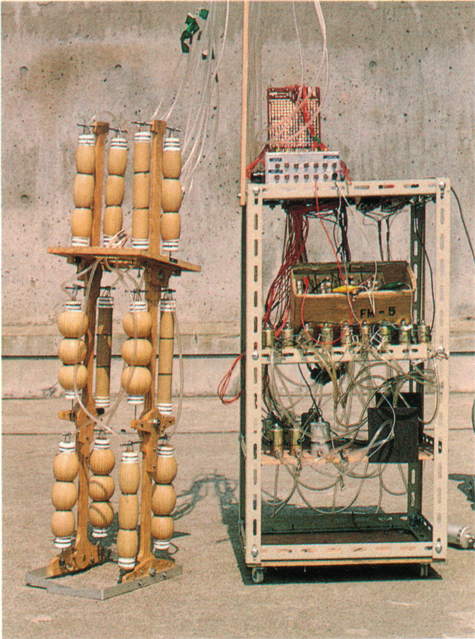
\includegraphics[scale=0.6]{imagenes/apartado_2/210_1_WAP_1_1969}}
\quad
\subfigure[WAP-2]
{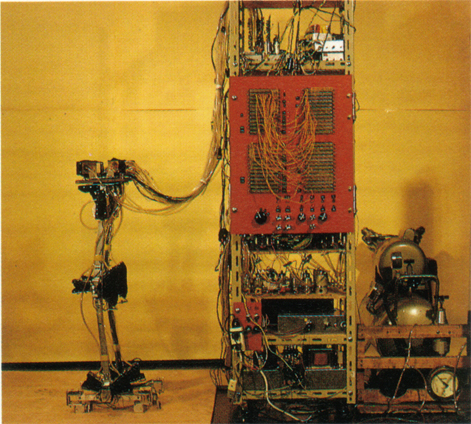
\includegraphics[scale=0.8]{imagenes/apartado_2/210_2_WAP_2_1970}}
\quad
\subfigure[WAP-3]
{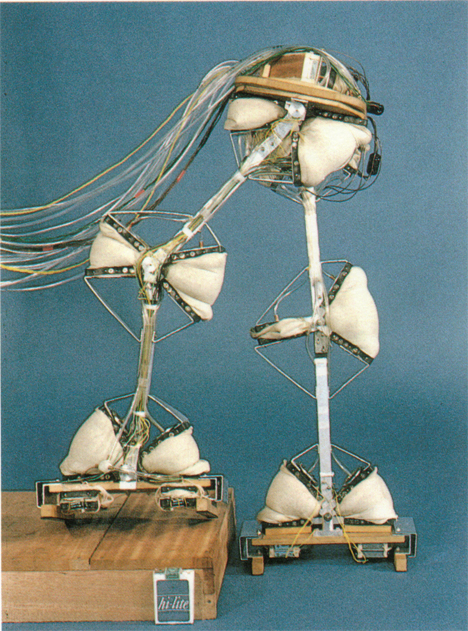
\includegraphics[scale=0.6]{imagenes/apartado_2/210_3_WAP_3_1971}}
\caption{Waseda's Anthropomorphic Pneumatically-activated pedipulators}
\label{figura210}
\end{figure}

Ya en 1970, con los avances en la investigación de robots antropomórficos inteligentes, aparecieron los primeros robots con torso y piernas, pareciéndose cada vez más a los seres humanos. De estos avances se desarrollaron los robots de la familia WABOT (WAseda roBOT), basados en sistemas de control de extremidades, visión y sistemas de conversación. El WABOT-2 incluso era capaz de leer partituras y tocar un teclado.

\begin{figure}[H]
\centering
\subfigure[WABOT-1]
{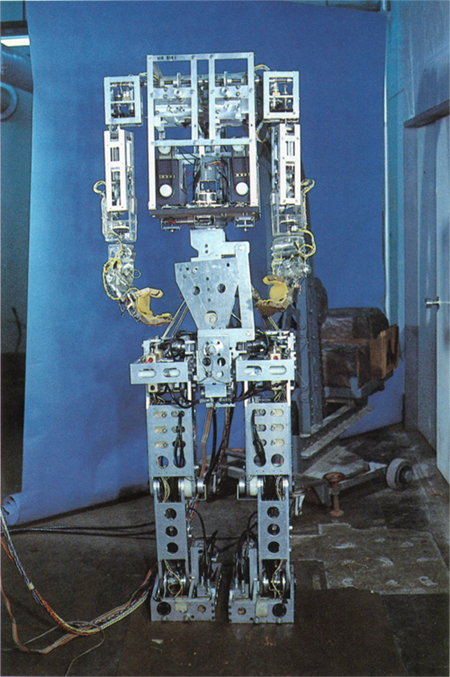
\includegraphics[scale=0.6]{imagenes/apartado_2/211_1_WABOT_1_1973}}
\quad
\subfigure[WABOT-2]
{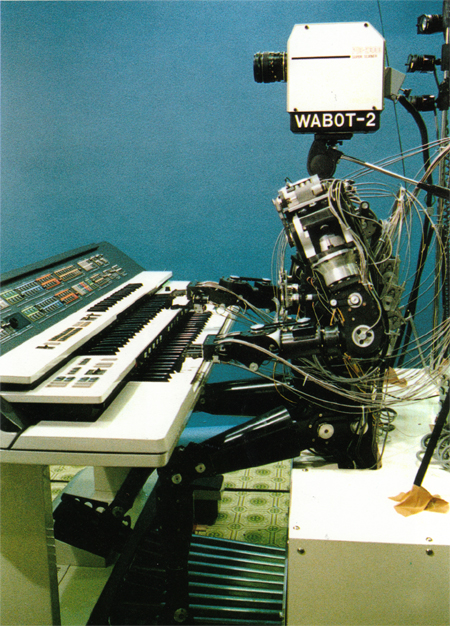
\includegraphics[scale=0.65]{imagenes/apartado_2/211_2_WABOT_2_1984}}
\caption{Robots antropomórficos inteligentes WAseda roBOT}
\label{figura211}
\end{figure}

Unos años más tarde, en 1996 se desarrolló la familia de robots WABIAN, que se caracterizaban por utilizar motores eléctricos, logrando la misma velocidad de paso que un humano \cite{ref8}.

En Japón la compañía HONDA llevaba desarrollando robots bípedos desde 1986. Primero fueron del modelo E0 al E6, para pasar a los P1 a P3 y terminando por el robot humanoide más inteligente llamado ASIMO, que fue desarrollado en el 2000.

\begin{figure}[H]
\centering
{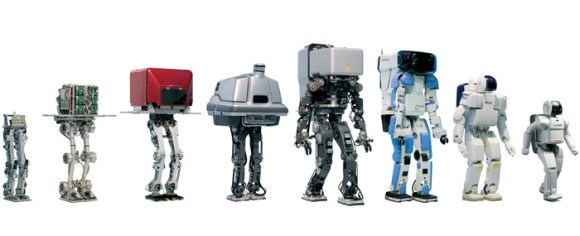
\includegraphics[scale=0.7]{imagenes/apartado_2/212_evolucion_Honda_robots}}
\caption{De izquierda a derecha, E0 hasta ASIMO}
\label{figura212}
\end{figure}

Dos años más tarde, bajo el Ministerio de Económicas, Comercio e Industria de Japón, se desarrolló el Proyecto Humanoide Robot (HRP), con el HRP-2 a la cabeza de la tecnología en esos años.

\begin{figure}[H]
\centering
{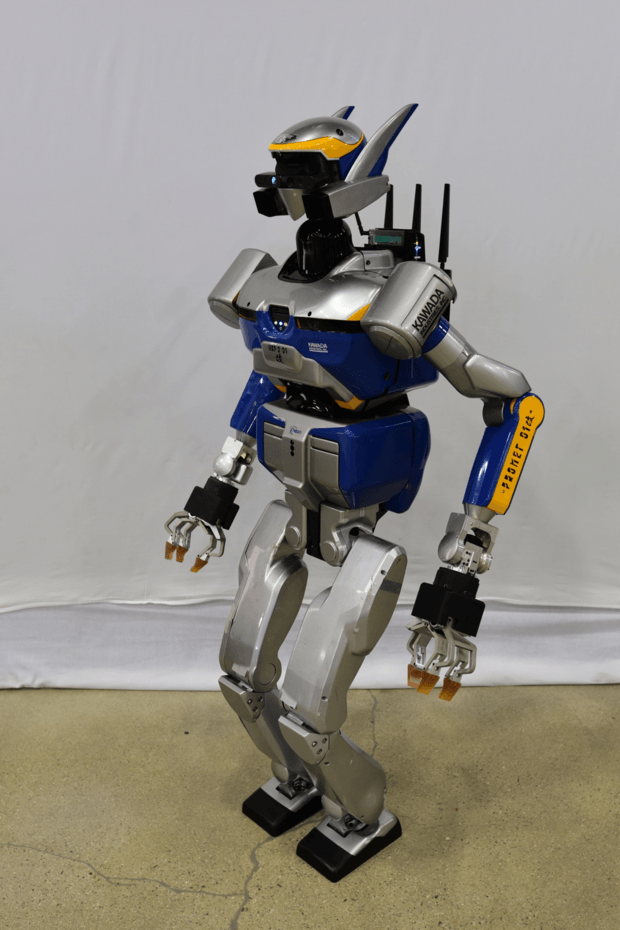
\includegraphics[scale=0.2]{imagenes/apartado_2/213_HRP_2}}
\caption{HRP-2}
\label{figura213}
\end{figure}

En la actualidad, los robots humanoides están muy avanzados, pudiendo incluso correr y mantener el equilibrio. Un ejemplo de ello lo tenemos en ATLAS, desarrollado en 2013 por Boston Dynamics, capaz de caminar por terrenos irregulares sin perder el equilibrio, cargar objetos pesados, e incluso recientemente, dar saltos.

\begin{figure}[H]
\centering
{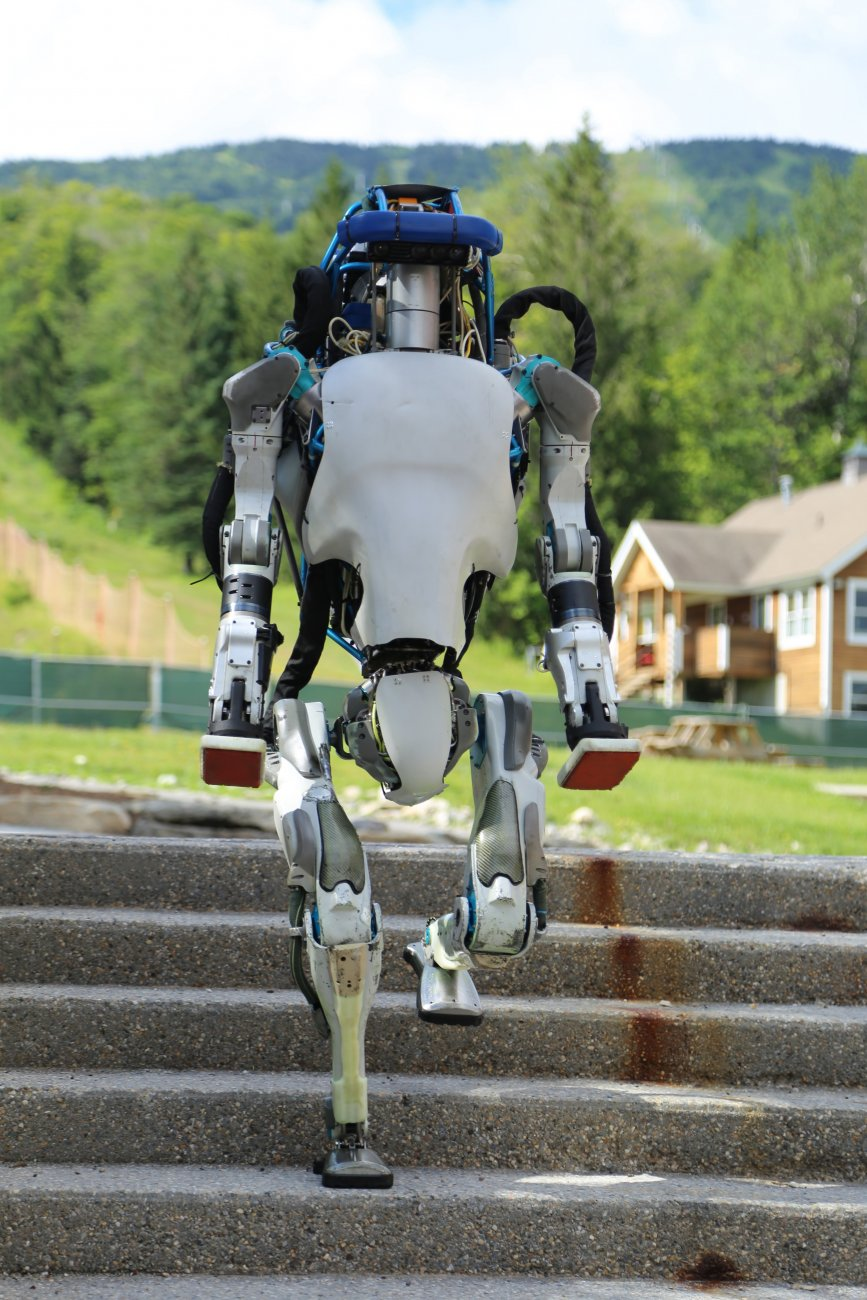
\includegraphics[scale=0.2]{imagenes/apartado_2/214_atlas_boston_dynamics}}
\caption{ATLAS}
\label{figura214}
\end{figure}

\newpage

\subsection{Locomoción bípeda}
%%Definición de centro de masas sacada de http://www2.montes.upm.es/dptos/digfa/cfisica/dinamsist/cdm.html
Para hablar de locomoción bípeda o caminata, primero hay que hacer una introducción de una serie de conceptos para poder entender mejor este movimiento.

\begin{itemize}
\item \emph{Centro de Masas} (CoM): es el punto en el que se concentra toda la masa del sistema y sobre el que actúa la resultante de todas las fuerzas que afectan al sistema \cite{ref9}.

\begin{figure}[H]
\centering
{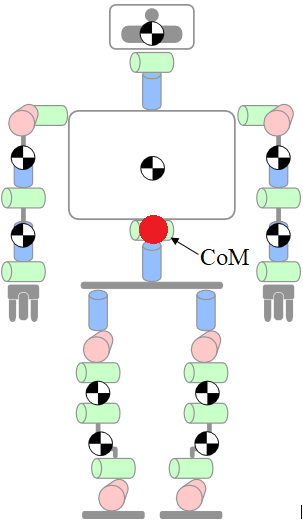
\includegraphics[scale=0.5]{imagenes/apartado_2/215_center_of_mass}}
\caption{Centro de Masas del robot humanoide TEO(en color rojo)}
\label{figura215}
\end{figure}

\item \emph{Polígono de soporte}: se trata del área de contacto de los puntos de apoyo con el suelo. Puede ser simple, con un pie, o doble, con los dos pies.

\begin{figure}[H]
\centering
{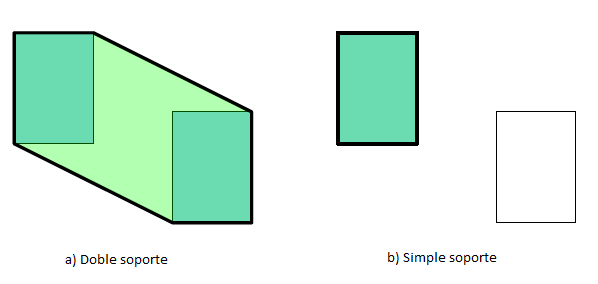
\includegraphics[scale=0.6]{imagenes/apartado_2/216_supportpolygon}}
\caption{Polígono de soporte}
\label{figura216}
\end{figure}

\item \emph{Punto de Momento Cero} (ZMP): Según Vukobratović \cite{ref19}, es el punto en el cual la suma de momentos es igual a 0.

\begin{figure}[H]
\centering
{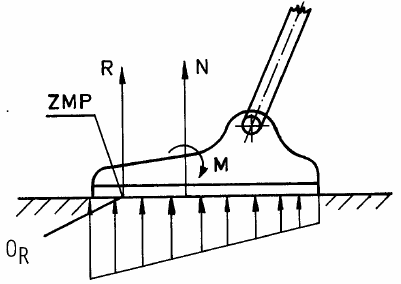
\includegraphics[scale=0.6]{imagenes/apartado_2/217_zmp}}
\caption{ZMP}
\label{figura217}
\end{figure}

\item \emph{Centro de Presión} (CoP): Punto en el polígono de soporte donde actúa la suma total de las fuerzas de contacto $R$, causando una fuerza pero no un momento.
%%Definición sacada de ZERO MOMENT POINT MaartenDekker_OPEN2009_Zero_Moment_Point_Method_for_Stable_Biped_Walking

\begin{figure}[H]
\centering
{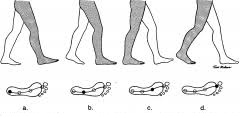
\includegraphics[scale=1.3]{imagenes/apartado_2/218_cop}}
\caption{Evolución del CoP durante el paso}
\label{figura218}
\end{figure}

\item \emph{Pivote del Momento Centroidal} (CMP): Punto donde la fuerza de reacción del suelo debería actuar para mantener constante la componente horizontal del momento angular de todo el cuerpo. El CMP es igual al ZMP en el caso en que el momento del CoM es cero. Sin embargo, cuando aparece un momento significativo sobre el CoM, aunque por definición el ZMP no puede abandonar el polígono de soporte en el suelo, el CMP puede hacerlo, como se puede observar en la imagen \ref{figura219}.

\begin{figure}[H]
\centering
{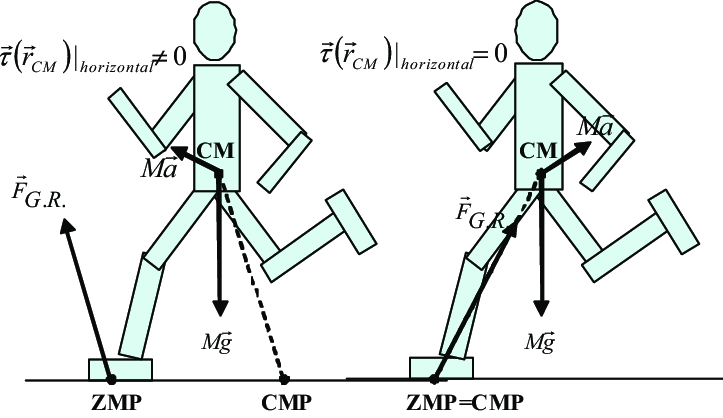
\includegraphics[scale=0.4]{imagenes/apartado_2/219_centroidal_moment_pivot}}
\caption{Pivote del Momento Centroidal (CMP)}
\label{figura219}
\end{figure}

\end{itemize}

\textbf{¿QUÉ ES LOCOMOCIÓN BÍPEDA O CAMINATA?}

La locomoción bípeda, o caminata, es la acción de desplazarse de un lugar a otro manteniendo en todo momento un pie en contacto con la superficie. En lo seres humanos este movimiento complejo y periódico alterna una fase de estabilidad con una fase de inestabilidad. Esta fase de inestabilidad es provocada por la gravedad, pero gracias a ella se produce el movimiento hacia adelante. Debido a la complejidad de este movimiento, se ha utilizado el criterio de Punto de Momento Cero (ZMP) para simplificar su análisis. 

Los robots humanoides han sido desarrollados para imitar los movimientos y comportamientos de los humanos. Pero la caminata resulta un comportamiento muy complejo para éstos. 

Existen dos tipos de caminata, llamadas caminata estática y  caminata dinámica. En la caminata estática el CoM no abandona nunca el polígono de soporte. Sin embargo, en la caminata dinámica, hay periodos en los que la proyección del CoM se sale fuera del polígono de soporte \cite{ref10}, como se puede observar en la Figura \ref{figura220}.

\begin{figure}[H]
\centering
{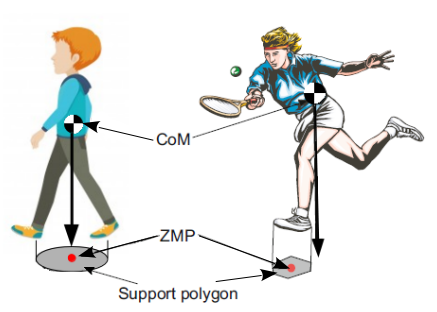
\includegraphics[scale=0.6]{imagenes/apartado_2/220_com_zmp_supportpolygon}}
\caption{CoM, Polígono de soporte y ZMP}
\label{figura220}
\end{figure}

Cuando los seres humanos realizan el movimiento de caminar logran mantener el equilibrio gracias a un control corporal total. Sin embargo los robots humanoides no son capaces de controlar por sí solos su cuerpo, por lo que su control de estabilidad es más complejo. En el actual proyecto se van a explicar dos modelos que desarrollan un controlador para mantener el equilibrio en los robots: el modelo de péndulo invertido y el modelo cart-table. Éstos consisten en calcular ciertos parámetros haciendo uso de los sensores de fuerza-par, en el caso del péndulo invertido, y del sensor inercial, en el caso del cart-table, para lograr mantener el equilibrio en la caminata de los robots.

\textbf{FASES DEL PASO}

En el paso o caminata bípeda, como se puede observar en la figura \ref{figura221}, las fases se distinguen por:

\begin{itemize}
\item \textbf{FASE 1}.Fase de apoyo\\
En esta fase la pierna y el pie que están completamente apoyados en el suelo, soportan todo el peso del bípedo, mientras la pierna de balanceo está realizando el paso.

\item \textbf{FASE 2}.Fase de balanceo\\
En esta fase la pierna y el pie que estaban antes apoyados ahora están realizando un paso (avanzando por el aire), hasta volver al apoyo de nuevo. 

\end{itemize}

\begin{figure}[H]
\centering
{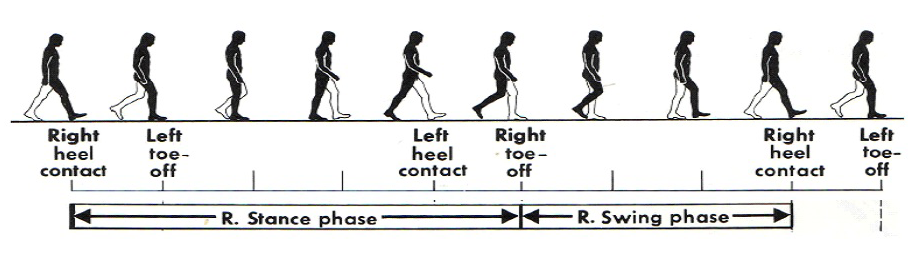
\includegraphics[scale=0.63]{imagenes/apartado_2/221_ciclo_paso_humano}}
\caption{Representación gráfica del paso o caminata}
\label{figura221}
\end{figure}

\newpage

\subsection{Zero Moment Point (ZMP)}

Vukobratović \cite{ref16} fue uno de los primeros en introducir el concepto más importante y principal a la hora de mantener el equilibrio de los robots humanoides bípedos. Decía que durante el paso, aparte de la realización del movimiento relativo entre juntas del mecanismo, la tarea más importante es preservar el equilibrio dinámico. Para ello toda el área del pie (incluyendo sus bordes) debe estar en contacto con el suelo.

\begin{figure}[H]
\centering
{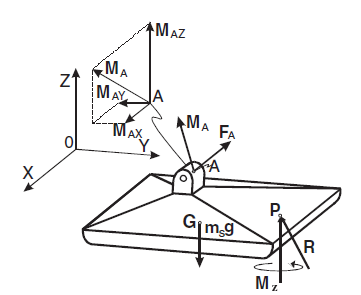
\includegraphics[scale=0.6]{imagenes/apartado_2/222_fuerzas_momentos}}
\caption{Representación de fuerzas y momentos que actúan sobre el pie de apoyo}
\label{figura222}
\end{figure}

Si el mecanismo está en equilibrio quiere decir que en el punto P de la suela, donde actúan las fuerzas de reacción del suelo,

\begin{equation}
\begin{split}
Mx=0\\
My=0
\end{split}
\label{ec21}
\end{equation}

Gracias a ello el punto P pasó a denominarse Punto de Momento Cero (ZMP), pudiéndose reducir dichas fuerzas a una sola llamada $R$ y a la componente z del momento $M_z$ sobre dicho punto.

Para calcular dicho punto y asegurarse de que el mecanismo está en equilibrio dinámico, teniendo en cuenta la dinámica del mecanismo, el requisito indispensable es que el pie esté completamente apoyado en el suelo. Para ello hay que partir de las ecuaciones del equilibrio estático para el pie de apoyo:

%%Ecuaciones 2 y 3
\begin{equation}
R+F_A+m_sg=0
\label{ec22}
\end{equation}
\begin{equation}
\overrightarrow{OP} \times \overrightarrow{R}+\overrightarrow{OG} \times m_sg + M_A+M_Z+\overrightarrow{OA} \times F_A=0
\label{ec23}
\end{equation}

donde $\overrightarrow{OP}$, $\overrightarrow{OG}$ y $\overrightarrow{OA}$ son los vectores desde el origen del sistema de coordenadas $O_(xyz)$ al punto P donde actúan las fuerzas de reacción del suelo, el centro de masas del pie (G), la articulación del tobillo (A), y la masa del pie $m_s$.

Dando su proyección en el plano horizontal se obtiene:

%%aquí va la eq 4.
\begin{equation}
(\overrightarrow{OP} \times \overrightarrow{R})^H+\overrightarrow{OG} \times m_sg+ (M_A)^H+(\overrightarrow{OA} \times F_A)^H=0 
\label{ec24}
\end{equation}

Esta ecuación permite calcular la posición del punto de actuación de la fuerza de reacción del suelo (P) para la dinámica general del mecanismo. Sin embargo esto no sirve para saber si está en equilibrio dinámico cuando el sistema está en movimiento. Para ello hay que tener en cuenta el punto P calculado y el polígono de soporte. Como el punto P calculado con ec \eqref{ec24} nunca puede existir fuera del polígono de soporte, ya que si lo hiciera la fuerza total R no actuaría sobre el sistema, sólo si éste está dentro del polígono de soporte el sistema estará en equilibrio dinámico.

Si suponemos que el punto P obtenido de $M_x=M_y=0$ está fuera del polígono de soporte, consideraríamos dicho punto como ZMP ficticio (\textbf{FZMP}). 

Ésto se puede explicar en el caso en el que el ZMP se está acercando al borde del polígono de soporte (tanto en simple soporte como en doble soporte). Si no hubiera más momentos adicionales, el sistema estaría en equilibrio (ZMP), pero si hay momentos adicionales el mecanismo comenzaría a girar y se colapsaría, ya que el punto de actuación de la fuerza de reacción del suelo estaría al borde del pie. Dicho punto ya no sería el ZMP.

Cuando el mecanismo está en movimiento, una manera de determinar el ZMP es midiendo las fuerzas que actúan cuando el pie entre en contacto con el suelo mediante sensores ubicados en la suela del mecanismo (todos los sensores deben estar en contacto con el suelo, ya que si no se cumple el mecanismo giraría en el borde del pie y volcaría), calculando dicho punto mediante el CoP, que se ha explicado anteriormente . Otra manera sería mediante un modelo dinámico. A partir de las fuerza y el momento en la articulación del tobillo ($F_A$ y $M_A$) el procedimiento para calcular ZMP consta de dos pasos:

\begin{enumerate}
\item Calcular $\overrightarrow{OP}$ de la ec \eqref{ec24}. La posición obtenida de P sería el ZMP. Aquí no sabemos todavía si el punto P se encuentra dentro o fuera del polígono de soporte porque no se tiene en cuenta el tamaño real de dicho polígono (figura \ref{figura223} a).

\item Una vez calculada la posición del ZMP, se compara con el tamaño real del polígono de soporte. Si está fuera significa que que el punto de actuación P de las fuerzas de reacción del suelo se encuentra en el borde del polígono de soporte y se poducirá una rotación del mecanismo debido al momento de desequilibrio, cuya intensidad depende de la distancia entre el borde del polígono de soporte y la posición del ZMP calculada, es decir, a la posición del FZMP. Si se encuentra dentro del polígono, el mecanismo estaría en equilibrio (figura \ref{figura223} b).

\begin{figure}[H]
\centering
\subfigure[]
{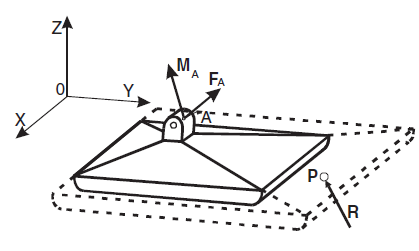
\includegraphics[scale=0.5]{imagenes/apartado_2/223_1_zmp}}
\quad
\subfigure[]
{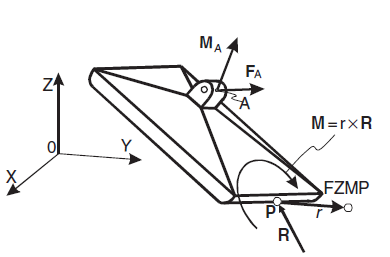
\includegraphics[scale=0.55]{imagenes/apartado_2/223_2_zmp}}
\caption{Determinación del ZMP}
\label{figura223}
\end{figure}

\end{enumerate}

\textbf{RELACIÓN ENTRE ZMP, FZMP Y COP}

Únicamente si la fuerza resultante $R$ está equilibrada con todas las fuerzas activas del sistema bípedo, el CoP y el ZMP coinciden, entonces podríamos decir que se encuentra en equilibrio dinámico, $P \equiv CoP \equiv ZMP$, como se muestra en la figura \ref{figura224}a. 

\begin{figure}[H]
\centering
\subfigure[Dinámicamente estable]
{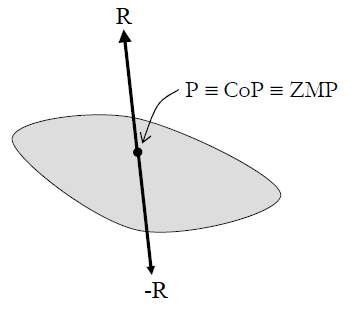
\includegraphics[scale=0.5]{imagenes/apartado_2/224_1_cop_zmp}}
\quad
\subfigure[Dinámicamente inestable]
{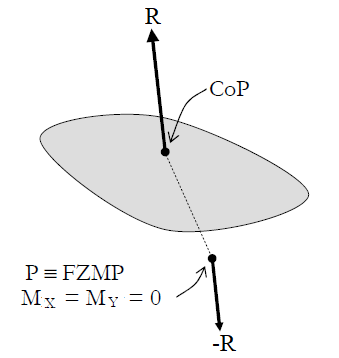
\includegraphics[scale=0.55]{imagenes/apartado_2/224_2_cop_zmp}}
\caption{Relación entre ZMP, FZMP y CoP}
\label{figura224}
\end{figure}

Sin embargo, si nos fijamos en la figura \ref{figura224}b vemos que el punto de ataque de las fuerzas cae fuera del soporte de apoyo, ZMP y CoP no coinciden, por lo que ahora $P \equiv FZMP$.

\afterpage{\null\newpage}
\newpage


